\begin{figure}[!tb]
    \centering
    % First Row
    \begin{minipage}{0.025\textwidth} % Narrow column for row label
        \raggedleft
        \rotatebox{90}{\text{RS}} % Vertical label for the first row
    \end{minipage}
    \begin{minipage}{0.06\textwidth}
        \centering
        
\includegraphics[width=\textwidth]{data_corrected/cam1_corrected/frame05.png}
        % \captionof{figure}{Rolling Shutter Image \(R_0\) where the corresponding Global Shutter image is at time \(t_0\)}

    \end{minipage}
    \begin{minipage}{0.06\textwidth}
        \centering
        
\includegraphics[width=\textwidth]{data_corrected/cam1_corrected/frame908.png}
        % \captionof{figure}{Rolling Shutter Image \(R_{N/2}\) where the corresponding Global Shutter image is at time \(t_{N/2}\)}
    \end{minipage}
    \begin{minipage}{0.06\textwidth}
        \centering
        
\includegraphics[width=\textwidth]{data_corrected/cam1_corrected/frame129.png}
        % \captionof{figure}{Rolling Shutter Image \(R_{N/2}\) where the corresponding Global Shutter image is at time \(t_{N/2}\)}
    \end{minipage}
    \begin{minipage}{0.06\textwidth}
        \centering
        
\includegraphics[width=\textwidth]{data_corrected/cam1_corrected/frame146.png}
        % \captionof{figure}{Rolling Shutter Image \(R_{N/2}\) where the corresponding Global Shutter image is at time \(t_{N/2}\)}
    \end{minipage}
    \begin{minipage}{0.06\textwidth}
        \centering
        
\includegraphics[width=\textwidth]{data_corrected/cam1_corrected/frame209.png}
        % \captionof{figure}{Rolling Shutter Image \(R_{N/2}\) where the corresponding Global Shutter image is at time \(t_{N/2}\)}
    \end{minipage}
    \begin{minipage}{0.06\textwidth}
        \centering
        
\includegraphics[width=\textwidth]{data_corrected/cam1_corrected/frame273.png}
        % \captionof{figure}{Rolling Shutter Image \(R_{N/2}\) where the corresponding Global Shutter image is at time \(t_{N/2}\)}
    \end{minipage}
    \begin{minipage}{0.06\textwidth}
        \centering
        
\includegraphics[width=\textwidth]{data_corrected/cam1_corrected/frame992.png}
        % \captionof{figure}{Rolling Shutter Image \(R_{N/2}\) where the corresponding Global Shutter image is at time \(t_{N/2}\)}
    \end{minipage}


    %second row
    \begin{minipage}{0.025\textwidth} % Narrow column for row label
        \raggedleft
        \rotatebox{90}{\text{GS}} % Vertical label for the first row
    \end{minipage}
       \begin{minipage}{0.06\textwidth}
        \centering
        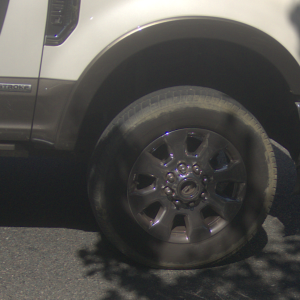
\includegraphics[width=\textwidth]{data_corrected/camera1/frame05.png}
        % \captionof{figure}{Rolling Shutter Image \(R_0\) where the corresponding Global Shutter image is at time \(t_0\)}

    \end{minipage}
    \begin{minipage}{0.06\textwidth}
        \centering
        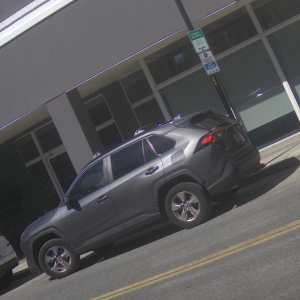
\includegraphics[width=\textwidth]{data_corrected/camera1/frame908.png}
        % \captionof{figure}{Rolling Shutter Image \(R_{N/2}\) where the corresponding Global Shutter image is at time \(t_{N/2}\)}
    \end{minipage}
    \begin{minipage}{0.06\textwidth}
        \centering
        
\includegraphics[width=\textwidth]{data_corrected/camera1/frame129.png}
        % \captionof{figure}{Rolling Shutter Image \(R_{N/2}\) where the corresponding Global Shutter image is at time \(t_{N/2}\)}
    \end{minipage}
    \begin{minipage}{0.06\textwidth}
        \centering
        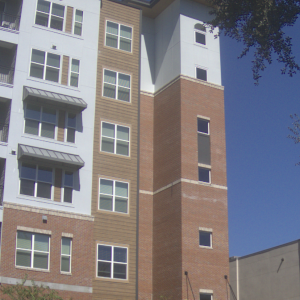
\includegraphics[width=\textwidth]{data_corrected/camera1/frame146.png}
        % \captionof{figure}{Rolling Shutter Image \(R_{N/2}\) where the corresponding Global Shutter image is at time \(t_{N/2}\)}
    \end{minipage}
    \begin{minipage}{0.06\textwidth}
        \centering
        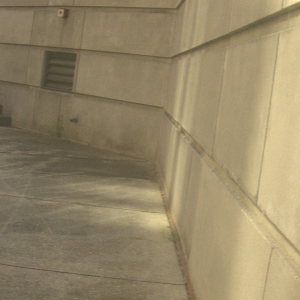
\includegraphics[width=\textwidth]{data_corrected/camera1/frame209.png}
        % \captionof{figure}{Rolling Shutter Image \(R_{N/2}\) where the corresponding Global Shutter image is at time \(t_{N/2}\)}
    \end{minipage}
    \begin{minipage}{0.06\textwidth}
        \centering
        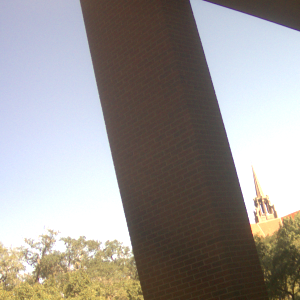
\includegraphics[width=\textwidth]{data_corrected/camera1/frame273.png}
        % \captionof{figure}{Rolling Shutter Image \(R_{N/2}\) where the corresponding Global Shutter image is at time \(t_{N/2}\)}
    \end{minipage}
    \begin{minipage}{0.06\textwidth}
        \centering
        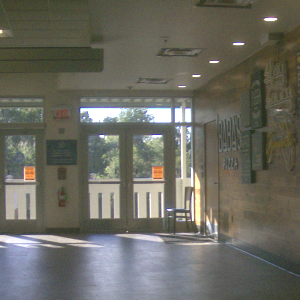
\includegraphics[width=\textwidth]{data_corrected/camera1/frame992.png}
        % \captionof{figure}{Rolling Shutter Image \(R_{N/2}\) where the corresponding Global Shutter image is at time \(t_{N/2}\)}
    \end{minipage}


    %Third Row
    \begin{minipage}{0.025\textwidth} % Narrow column for row label
        \raggedleft
        \rotatebox{90}{\text{RS}} % Vertical label for the first row
    \end{minipage}
       \begin{minipage}{0.06\textwidth}
        \centering
        
\includegraphics[width=\textwidth]{data_corrected/cam1_corrected/frame902.png}
        % \captionof{figure}{Rolling Shutter Image \(R_0\) where the corresponding Global Shutter image is at time \(t_0\)}

    \end{minipage}
    \begin{minipage}{0.06\textwidth}
        \centering
        
\includegraphics[width=\textwidth]{data_corrected/cam1_corrected/frame134.png}
        % \captionof{figure}{Rolling Shutter Image \(R_{N/2}\) where the corresponding Global Shutter image is at time \(t_{N/2}\)}
    \end{minipage}
    \begin{minipage}{0.06\textwidth}
        \centering
        
\includegraphics[width=\textwidth]{data_corrected/cam1_corrected/frame28.png}
        % \captionof{figure}{Rolling Shutter Image \(R_{N/2}\) where the corresponding Global Shutter image is at time \(t_{N/2}\)}
    \end{minipage}
    \begin{minipage}{0.06\textwidth}
        \centering
        
\includegraphics[width=\textwidth]{data_corrected/cam1_corrected/frame32.png}
        % \captionof{figure}{Rolling Shutter Image \(R_{N/2}\) where the corresponding Global Shutter image is at time \(t_{N/2}\)}
    \end{minipage}
    \begin{minipage}{0.06\textwidth}
        \centering
        
\includegraphics[width=\textwidth]{data_corrected/cam1_corrected/frame383.png}
        % \captionof{figure}{Rolling Shutter Image \(R_{N/2}\) where the corresponding Global Shutter image is at time \(t_{N/2}\)}
    \end{minipage}
    \begin{minipage}{0.06\textwidth}
        \centering
        
\includegraphics[width=\textwidth]{data_corrected/cam1_corrected/frame471.png}
        % \captionof{figure}{Rolling Shutter Image \(R_{N/2}\) where the corresponding Global Shutter image is at time \(t_{N/2}\)}
    \end{minipage}
    \begin{minipage}{0.06\textwidth}
        \centering
        
\includegraphics[width=\textwidth]{data_corrected/cam1_corrected/frame53.png}
        % \captionof{figure}{Rolling Shutter Image \(R_{N/2}\) where the corresponding Global Shutter image is at time \(t_{N/2}\)}
    \end{minipage}


    %fourth row
    \begin{minipage}{0.025\textwidth} % Narrow column for row label
        \raggedleft
        \rotatebox{90}{\text{GS}} % Vertical label for the first row
    \end{minipage}
   \begin{minipage}{0.06\textwidth}
        \centering
        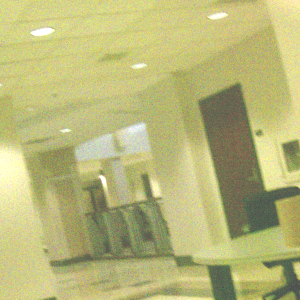
\includegraphics[width=\textwidth]{data_corrected/camera1/frame902.png}
        % \captionof{figure}{Rolling Shutter Image \(R_0\) where the corresponding Global Shutter image is at time \(t_0\)}

    \end{minipage}
    \begin{minipage}{0.06\textwidth}
        \centering
        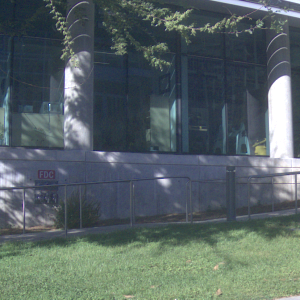
\includegraphics[width=\textwidth]{data_corrected/camera1/frame134.png}
        % \captionof{figure}{Rolling Shutter Image \(R_{N/2}\) where the corresponding Global Shutter image is at time \(t_{N/2}\)}
    \end{minipage}
    \begin{minipage}{0.06\textwidth}
        \centering
        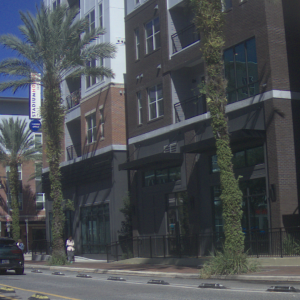
\includegraphics[width=\textwidth]{data_corrected/camera1/frame28.png}
        % \captionof{figure}{Rolling Shutter Image \(R_{N/2}\) where the corresponding Global Shutter image is at time \(t_{N/2}\)}
    \end{minipage}
    \begin{minipage}{0.06\textwidth}
        \centering
        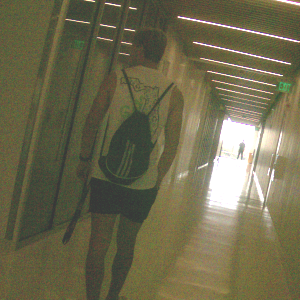
\includegraphics[width=\textwidth]{data_corrected/camera1/frame32.png}
        % \captionof{figure}{Rolling Shutter Image \(R_{N/2}\) where the corresponding Global Shutter image is at time \(t_{N/2}\)}
    \end{minipage}
    \begin{minipage}{0.06\textwidth}
        \centering
        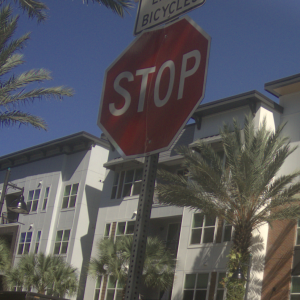
\includegraphics[width=\textwidth]{data_corrected/camera1/frame383.png}
        % \captionof{figure}{Rolling Shutter Image \(R_{N/2}\) where the corresponding Global Shutter image is at time \(t_{N/2}\)}
    \end{minipage}
    \begin{minipage}{0.06\textwidth}
        \centering
        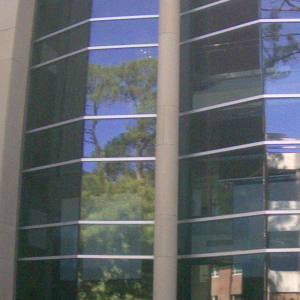
\includegraphics[width=\textwidth]{data_corrected/camera1/frame471.png}
        % \captionof{figure}{Rolling Shutter Image \(R_{N/2}\) where the corresponding Global Shutter image is at time \(t_{N/2}\)}
    \end{minipage}
    \begin{minipage}{0.06\textwidth}
        \centering
        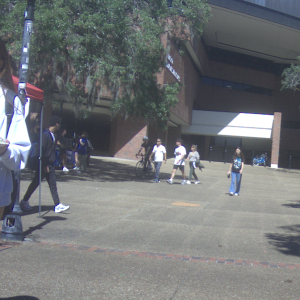
\includegraphics[width=\textwidth]{data_corrected/camera1/frame53.png}
        % \captionof{figure}{Rolling Shutter Image \(R_{N/2}\) where the corresponding Global Shutter image is at time \(t_{N/2}\)}
    \end{minipage}

    
    \caption{Highlights of the Real Dataset. Each pair of rows shows the rolling shutter capture and the corresponding global shutter capture. The dataset will be released to the public.}
    \label{fig:Real_Dataset}
    \vspace{-3mm}
\end{figure}
